\section{De JSON a JSON-LD}


Se consultó la API de la DNCP que sigue el formato de OCDS, a modo de ejemplo se utlizó el proceso de licitación numero 193399 a través de la siguiente URL https://www.contrataciones.gov.py/datos/api/v2/doc/ocds/record-package/193399 .

Se extrajo solamente el objeto Compiled Release, que posee toda la información del proceso licitatorio. Una versión resumida del objeto se puede visualizar en la Figura \ref{img:json1}. Se puede ver que el objeto tiene las siguientes propiedades: language, ocid, date, tag Initiation Type, planning, tender, buyer, awards, contracts.



\begin{figure}[h!]
    \centering
    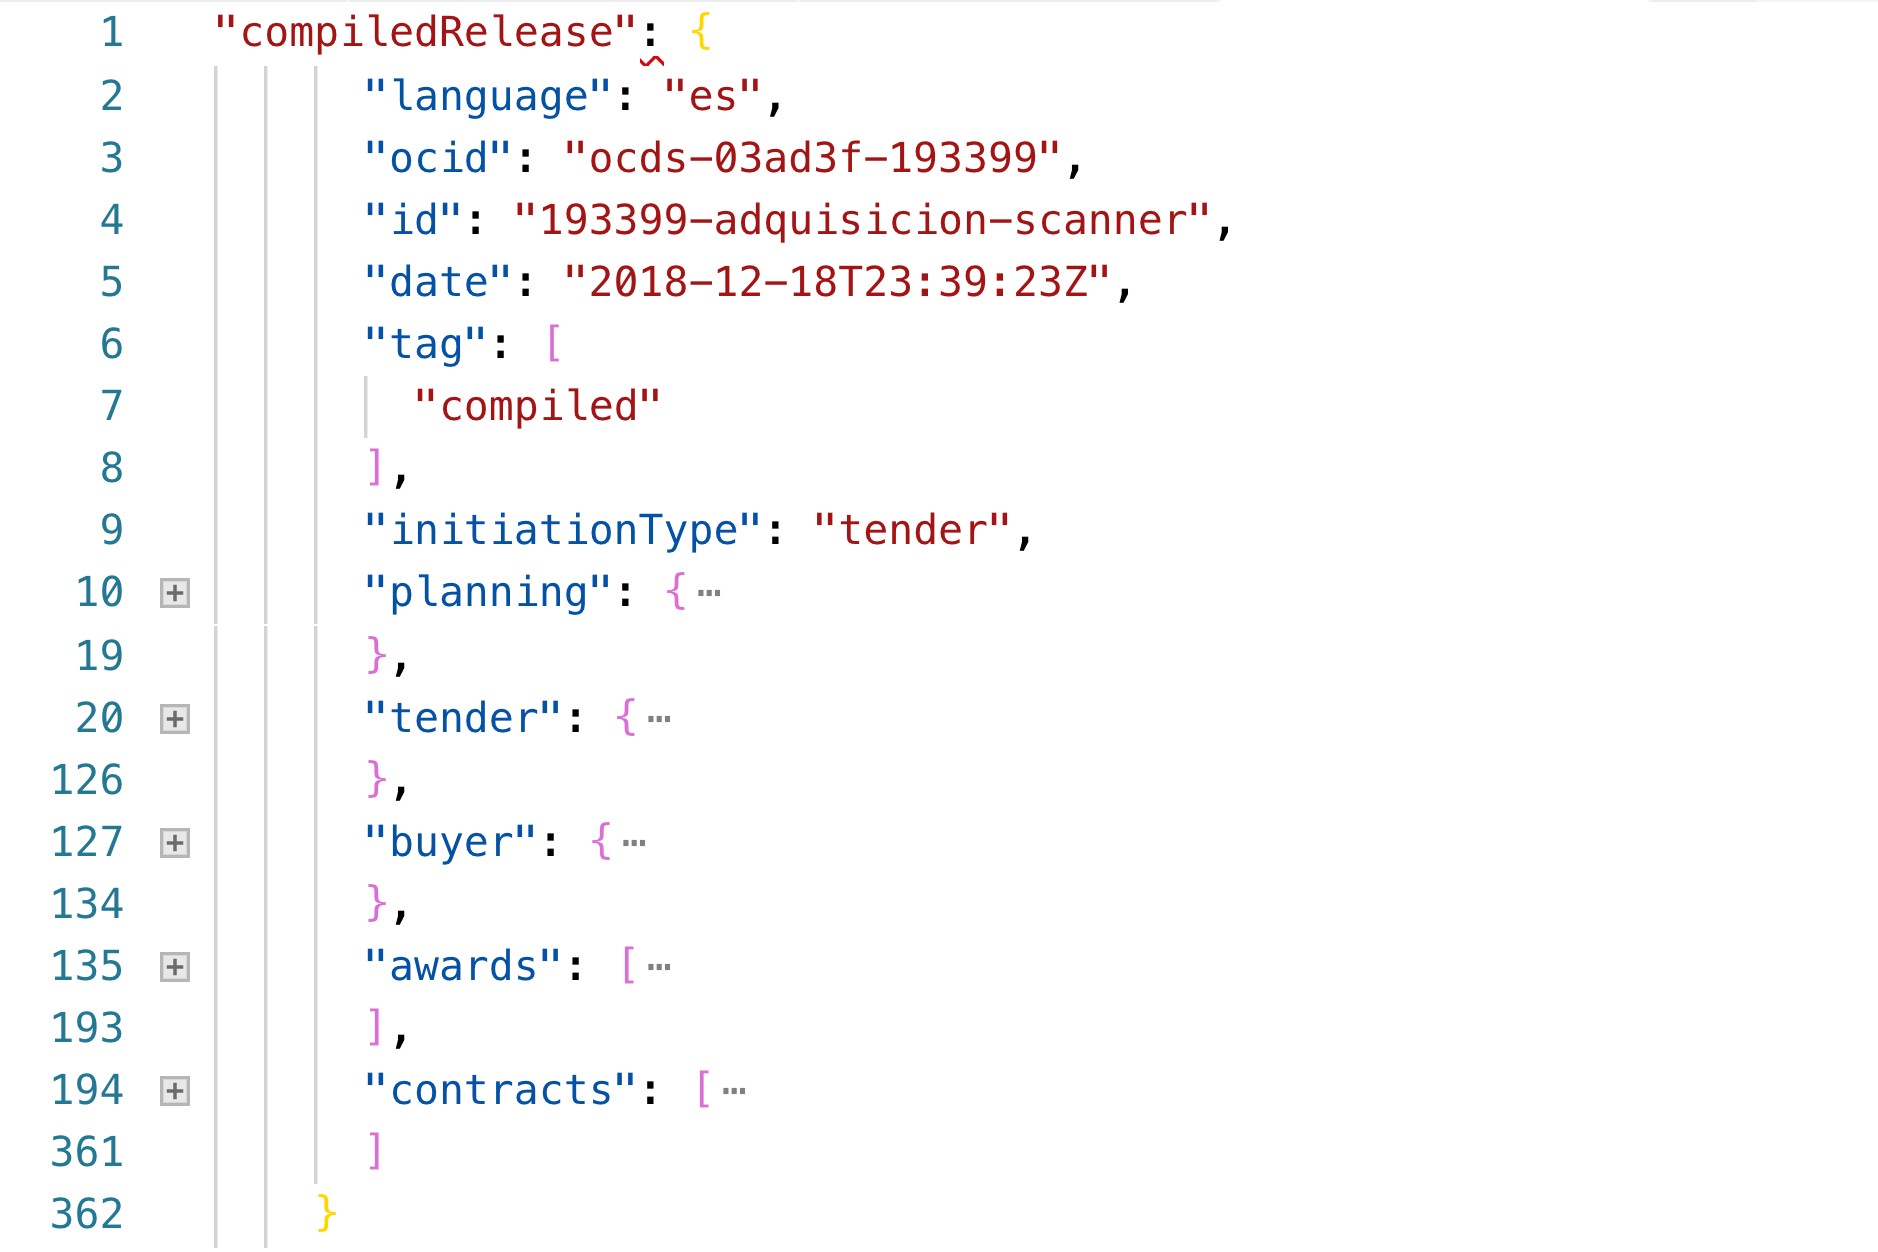
\includegraphics[width=150mm]{figuras/1}
    \caption{Objeto JSON del OCDS de un Compiled Release}
    \label{img:json1}
    \end{figure}



Para enriquecer semánticamente un objeto debemos agregar un contexto y los respectivos @id para poder convertirlo a JSON-LD. 

Nos encontramos con que no sería suficiente un solo contexto para todo el objeto. Esto se debe a las colisiones que existen entre propiedades que poseen el mismo nombre y distintos significados.

Dado que la definición de los contextos se da en forma de cascada, es decir se toma la definición más próxima, se definió un contexto para cada objeto hijo.

A continuación se muestra la colisión entre conceptos, donde amount (del objeto budget) se refiere al valor monetario (número y moneda) del presupuesto, y la siguiente propiedad amount (del objeto amount) se refiere al valor numérico específicamente.\hfill \break

\noindent\begin{minipage}{\textwidth}
\begin{lstlisting}[captionpos=b, caption=Objeto JSON con colisión semántica entre conceptos, label=lst:oJson,language=json,firstnumber=1,  numbers=left,  numberstyle=\tiny\color{mygray},
    basicstyle=\footnotesize\ttfamily,frame=single]
    "budget": {
        "description": "Adquisicion de Scanner",
        "amount": {
              "amount": 12000000,
              "currency": "PYG"
         }
     }  
    \end{lstlisting}
\end{minipage}
\noindent
\begin{minipage}{\textwidth}
    \begin{lstlisting}[captionpos=b, caption=Objeto JSON-LD. Sin colisión semántica entre conceptos , label=lst:oJsonLd, language=json,firstnumber=1,  numbers=left,  numberstyle=\tiny\color{mygray},
    basicstyle=\footnotesize\ttfamily,frame=single]
        "budget": {
            "@context": "http://purl.org/onto-ocds/ocds/context-budget.json",
            "@type": "Budget",
            "description": "Adquisicion de Scanner",
            "amount": {
                "@context": "http://purl.org/onto-ocds/ocds/context-value.json",
                "@type": "Value",
                "amount": 12000000,
                "currency": "PYG"
           }
       }   
        \end{lstlisting}
    \end{minipage}

        En el Cuadro \ref{lst:oJsonLd} se observa la solución implementada de manera a que el objeto “budget” tenga la definición de su atributo “amount” y el objeto “amount” tenga la definición de su atributo “amount” por separado evitando así inconsistencias.

A modo de ejemplo, se procedió a crear un contexto para el objeto planning que se muestra en la Figura \ref{img:json2} y todos los objetos hijos del mismo. En la Figura \ref{img:json3} se puede observar que se agregaron las propiedades @context en las líneas 2,6,10, la propiedad @type en las líneas 3,7,11 y la propiedad @id en la línea 4.

Se utilizó la herramienta JSON-LD PLAYGROUND \cite{JSONLDPl78:online} y RDF Translator \cite{RDFTrans0:online} para verificar la sintaxis de los documentos creados.

\begin{figure}[h!]
    \centering
    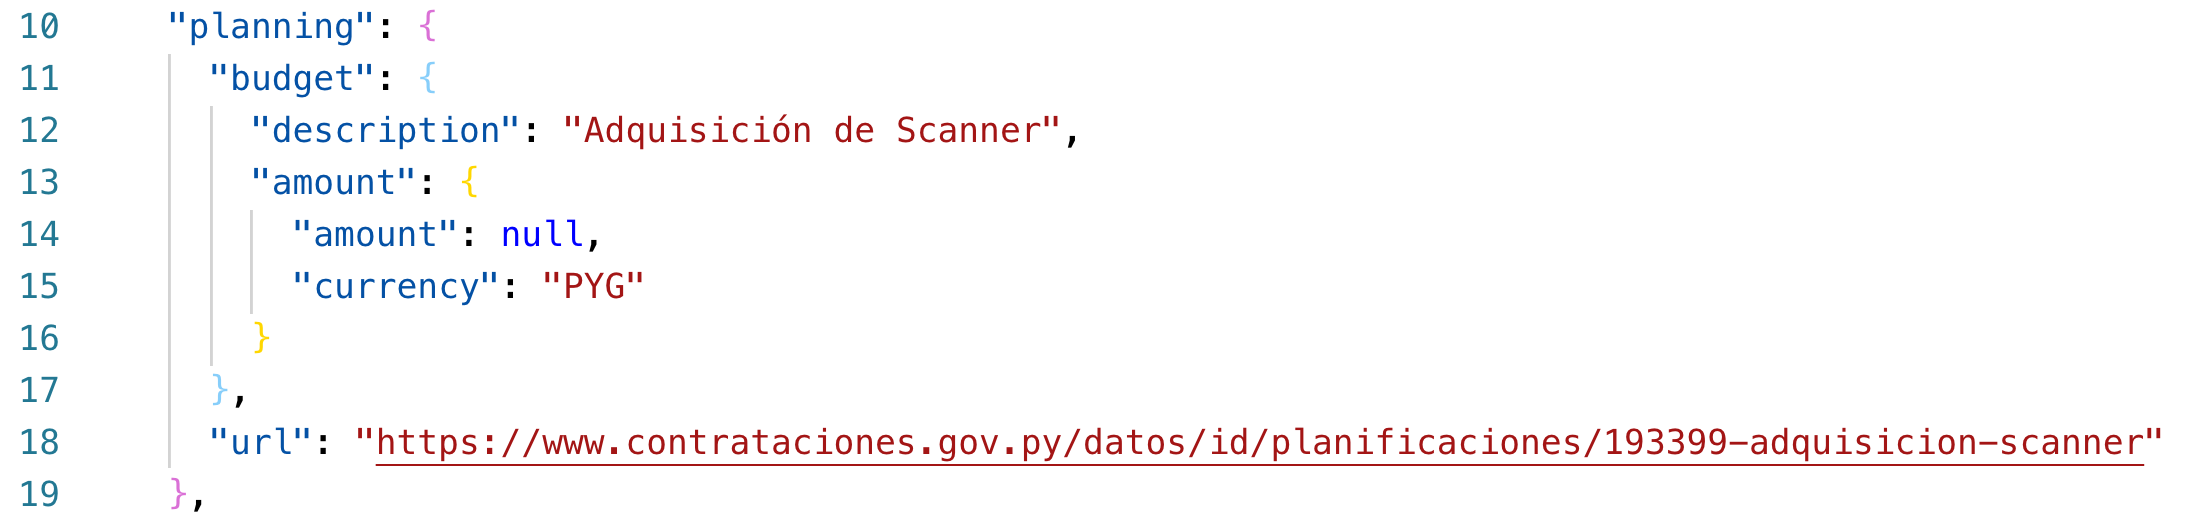
\includegraphics[width=150mm]{figuras/2}
    \caption{Objeto JSON del OCDS de un Planning}
    \label{img:json2}
    \end{figure}

\begin{figure}[h!]
    \centering
    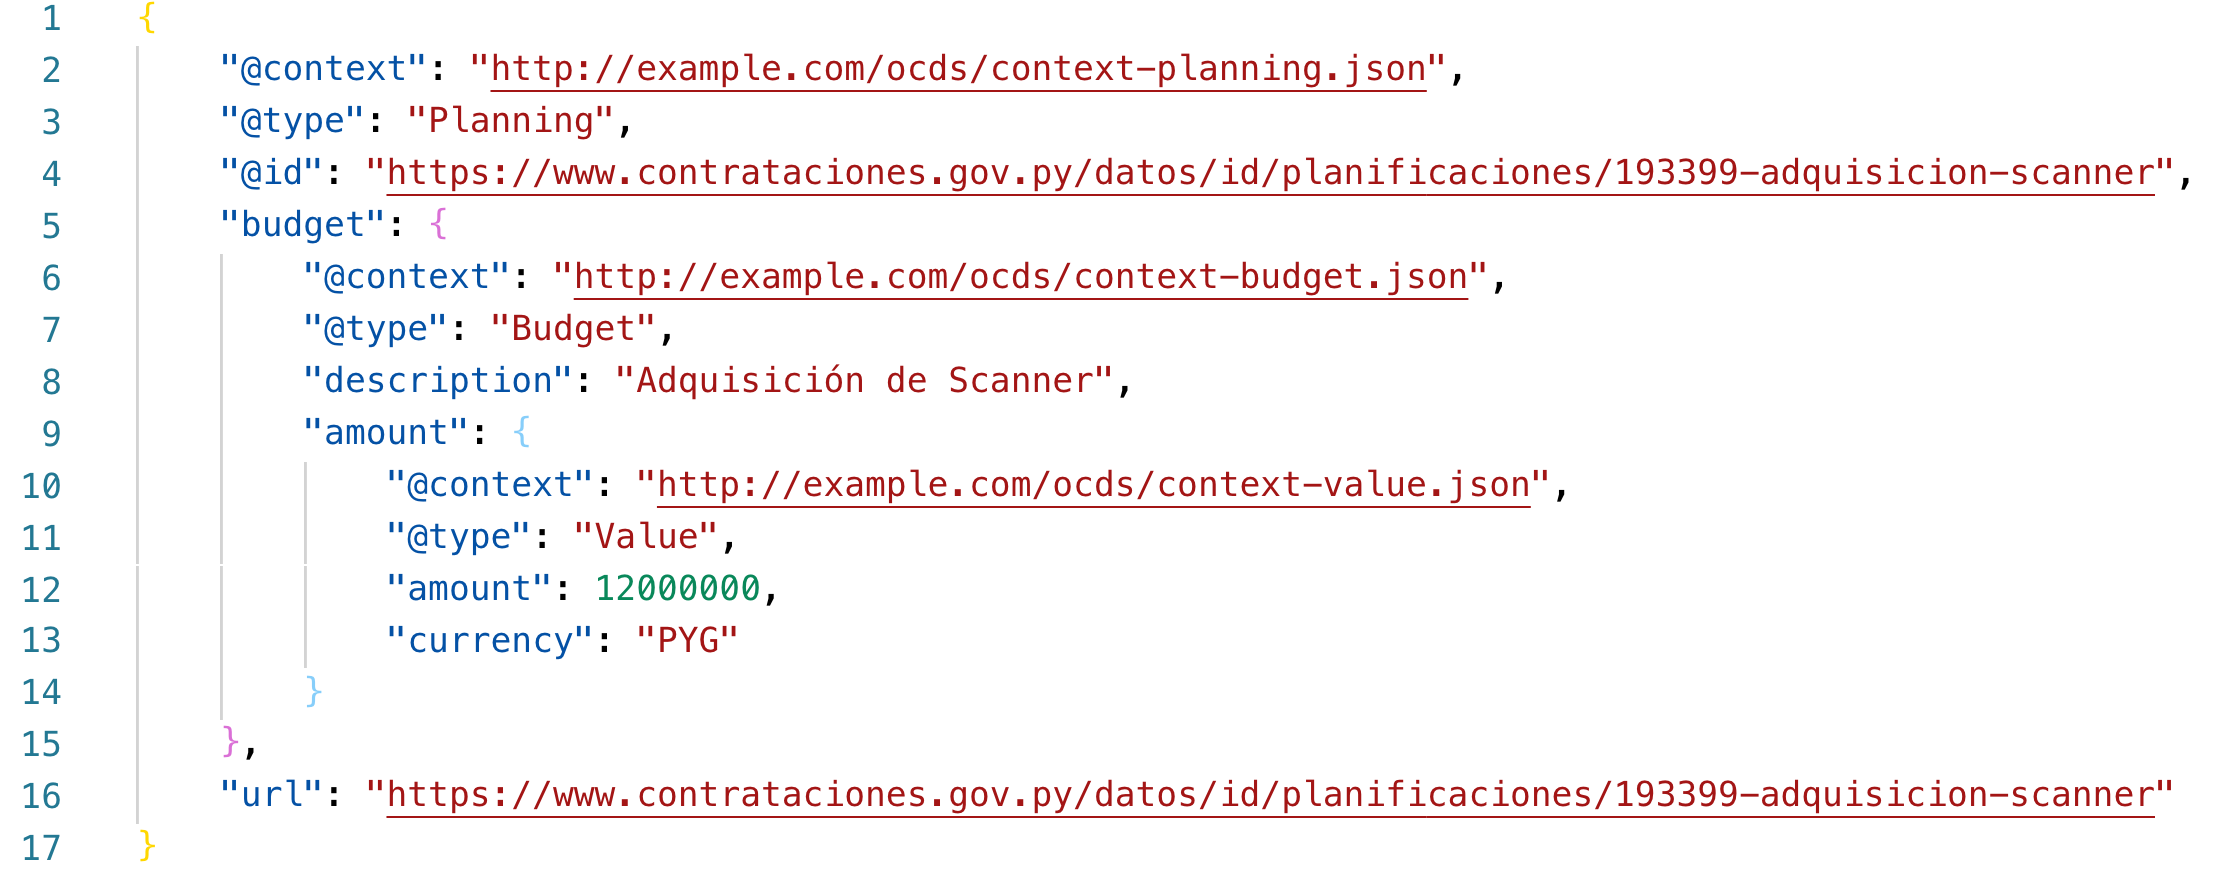
\includegraphics[width=150mm]{figuras/3}
    \caption{Objeto JSON-LD del OCDS de un Planning}
    \label{img:json3}
    \end{figure}


Los documentos de los contextos sirven para referenciar a cada propiedad con la ontología creada. En la Figura \ref{img:json4} se muestra el contenido del documento context-planning.json. Nótese de que sólo están definidas las propiedades hijas del objeto planning, los demás ancestros se encuentran definidas en el documento del padre.

Además solo se agrego la propiedad @id al objeto planning, el objeto amount no posee un @id debido a que la implementación de la DNCP tampoco provee un identificador único para ese objeto, esto significa que a la conversión a RDF de dicho objeto derivará en un Blank Node, por lo que no será posible referenciar dicha instancia más allá de este documento.


\begin{figure}[h!]
    \centering
    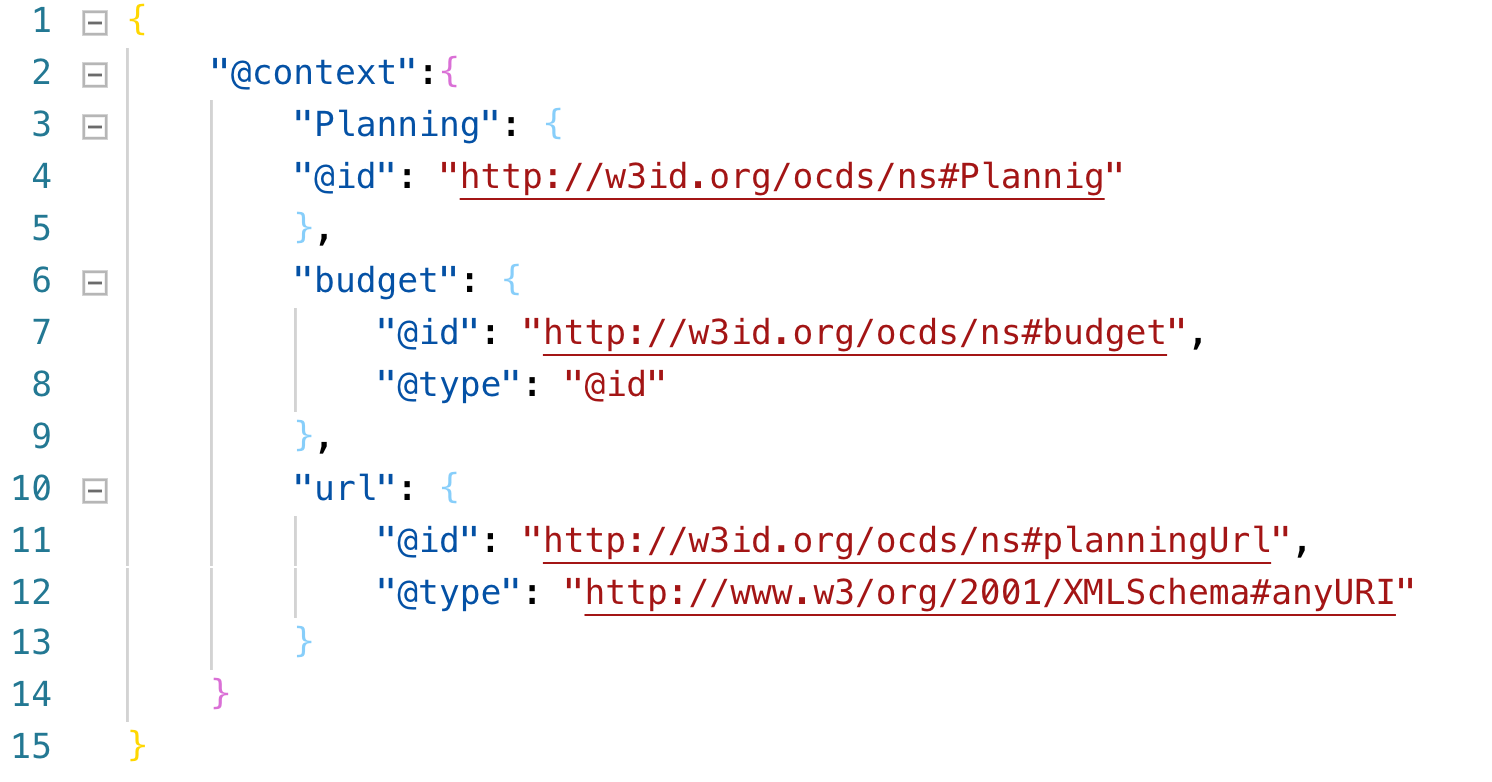
\includegraphics[width=150mm]{figuras/4}
    \caption{Contexto del Objeto Planning }
    \label{img:json4}
    \end{figure}


Un inconveniente al momento de generar los valores para los atributos del @id, es que los objetos no poseen un valor válido, en este caso una URI que desreferencie dicho objetos. El procedimiento consiste en verificar si el objeto posee un atributo “uri” cuyo valor sea una URI, de no ser el caso se procede a verificar si posee los atributos “url” e “id” sucesivamente. En el caso de que posea estos atributos pero con valores inválidos, osea no sean una URI propiamente dicha, se crea una ficticia a fin de que tenga un @id con formato válido. Si un objeto no tiene un @id válido, entonces no podrá ser convertido luego a formato RDF. Este fue el caso para los Items, Lotes.

Otra excepción fue el caso de los Codelist abiertos y cerrados. En cada caso se procedió a transformar el valor del atributo correspondiente, que en este caso era un String que no era una URI, a una URI que referencia a una instancia del respectivo CodeList. A modo de ejemplo se transformaron valores de los atributos de TenderStatus, AwardStatus, ContractStatus, Classification Scheme que referencian a las instancias que se encuentran en la ontología desarrollada. Los demás Codelist ya poseen las instancias respectivas dentro de la ontología desarrollada, pero la conversión de los mismos en los datos de la DNCP quedó como futuro trabajo.

Se realizó en mismo procedimiento con los demás objetos pertenecientes al JSON. Como futuro trabajo se podrá optimizar el tiempo de carga del documento JSON-LD agregando contextos sólo cuando exista una colisión semántica, de esta manera se ahorrarán líneas

Como siguiente paso nos queda convertir de manera programática los objetos publicados en JSON a JSON-LD para su posterior serialización a RDF.

